%generare il pdf con il comando: pdflatex main.tex
\documentclass[a4paper, oneside, openany]{article}
\usepackage{../template/sos}
\newcommand{\Titolo}{Norme di Progetto}

\newcommand{\Gruppo}{SonsOfSwe}

\newcommand{\Redazione}{Caldart Federico, Cavallin Giovanni, Dalla Riva Giovanni, Favero Andrea, Menegon Lorenzo, Panozzo Stefano, Thiella Eleonora}

\newcommand{\ACapoRedazione}{Caldart Federico \newline Cavallin Giovanni \newline Dalla Riva Giovanni \newline Favero Andrea \newline Menegon Lorenzo \newline Panozzo Stefano \newline Thiella Eleonora}

\newcommand{\Verifica}{Caldart Federico}

\newcommand{\Approvazione}{Cavallin Giovanni}

\newcommand{\Distribuzione}{Vardanega Tullio}

\newcommand{\Uso}{interno}

\newcommand{\Data}{3 Marzo 2018}

\newcommand{\NomeProgetto}{Progetto Speect}

\newcommand{\Mail}{sonsofswe.swe@gmail.com}

\newcommand{\DescrizioneDoc}{Questo documento descrive le regole, gli strumenti e le convenzioni adottate dal gruppo SonsOfSwe durante la realizzazione del progetto Marvin.}



\begin{document}
\copertina{}
%%%%%%%%%%%%%%%%%%%%%%%%%%%%%%%%%%%%%%%%%%%%%%%%%%%%%%%%%%%%%%%%%%%%%%%%%%%%%%%%%%%%%%%%%%%%%%%%%%%%%%%
%SOMMARIO
\tableofcontents
\newpage
%%%%%%%%%%%%%%%%%%%%%%%%%%%%%%%%%%%%%%%%%%%%%%%%%%%%%%%%%%%%%%%%%%%%%%%%%%%%%%%%%%%%%%%%%%%%%%%%%%%%%%%
%PARAGRAFI
\newpage
\section{Introduzione}
\subsection{Scopo del documento}
Questo documento contiene la pianificazione delle attività che saranno svolte dai membri del gruppo \Gruppo{} per realizzare il progetto \NomeProgetto. In particolare, questo documento contiene:

\begin{itemize}
	\item Analisi e trattamento dei rischi;
	\item Il preventivo delle risorse necessarie allo svolgimento del progetto;
	\item Il consuntivo delle attività finora svolte.
\end{itemize}

\subsection{Scopo del prodotto}
Lo scopo del prodotto è quello di realizzare un prototipo di Uniweb come ÐApp che giri su rete Ethereum. I tre attori principali che si rapportano con Marvin sono:
\begin{itemize}
	\item Università;
	\item Professori;
	\item Studenti.
\end{itemize} 
Il portale deve quindi permettere agli studenti di accedere alle informazioni riguardanti le loro carriere universitarie, di iscriversi agli esami, di accettare o rifiutare voti e di poter vedere il loro libretto universitario.
Ai professori deve invece essere permesso registrare i voti degli studenti.
L'università ogni anno crea una serie di corsi di laurea rivolti a studenti, dove ognuno di essi comprende un elenco di esami disponibili per anno accademico. Ogni esame ha un argomento, un numero di crediti e un professore associato. Gli studenti si iscrivono ad un corso di laurea e tramite il libretto elettronico mantengono traccia ufficiale del progresso.

\subsection{Glossario}
Nel documento \textit{Glossario} i termini tecnici, gli acronimi e le abbreviazioni sono definiti in modo chiaro e conciso, in modo tale da evitare ambiguità e massimizzare la comprensione dei documenti.
\newline I vocaboli presenti in esso saranno posti in corsivo e presenteranno una "G" maiuscola a pedice.

\subsection{Riferimenti}
\subsubsection{Normativi}
\begin{itemize}
	\item \textbf{Norme di Progetto: }\textit{Norme di Progetto v1.0.0};
	\item \textbf{Capitolato d'appalto C6: \NomeProgetto}:\\
	\url{http://www.math.unipd.it/~tullio/IS-1/2017/Progetto/C6.pdf};
	\item \textbf{Regolamento del progetto didattico}:\\
	\url{http://www.math.unipd.it/~tullio/IS-1/2017/Dispense/P01.pdf};
	\item \textbf{Vincoli di organigramma e dettagli tecnico-economici}:\\
	\url{http://www.math.unipd.it/~tullio/IS-1/2017/Progetto/RO.html}.
\end{itemize}
\subsubsection{Informativi}
\begin{itemize}
	\item \textbf{Studio di Fattibilità: }\textit{Studio di Fattibilità v1.0.0};
	\item \textbf{Analisi dei Requisiti: }\textit{Analisi dei Requisiti v1.0.0};
	\item \textbf{Software Engineering (10th edition) - Ian Sommerville}:
	\begin{itemize}
		\item Chapter 2: Software processes;
		\item Chapter 22: Project management;
		\item Chapter 23: Project Planning.
	\end{itemize}
	\item \textbf{Slides del corso di Ingegneria del Software}:\\
	\url{http://www.math.unipd.it/~tullio/IS-1/2017/}.
\end{itemize}

\subsection{Modello di sviluppo}
Il modello di sviluppo scelto per il progetto è quello incrementale.\\
Durante i primi periodi, grazie ad un'analisi del capitolato e la comunicazione con il proponente, si fissano i requisiti che il sistema dovrà soddisfare e quali invece sono considerati opzionali, benchè desiderabili. Questo permette di individuare quali dei requisiti hanno una maggior importanza strategica; pertanto questi verranno soddisfatti per primi, mentre gli altri saranno adempiti successivamente.\\
Il modello infatti prevede rilasci multipli successivi, dunque è possibile sottoporre al proponente un prototipo con le funzionalità di primaria importanza nel minor tempo possibile, così da permettere una valutazione in corso d’opera del lavoro svolto. Partendo da questo prototipo sarà poi possibile effettuare un incremento delle funzionalità e un consolidamento di quelle già presenti.\\
Per ottenere ciò nel modo più efficiente ed efficace possibile, si prevede la scomposizione dello sviluppo in attività, al termine delle quali è prevista una milestone (interna o esterna). In questo modo le risorse vengono concentrate in un numero limitato di sottoattività parallele, ottenendo come risultato una loro migliore gestione e verifica.
Questo permette un maggiore controllo sulle tempistiche e sui costi in quanto ogni sottoinsieme deve essere precedentemente pianificato; ciò riduce inoltre il rischio di ritardi.\\
Infine, per ogni attività si prevedono dei giorni di slack prima della consegna dei documenti per accedere alle revisioni di avanzamento, in modo da mitigare eventuali ritardi causati da fattori non prevedibili.

\subsection{Scadenze}\label{Scadenze}
Il gruppo \Gruppo ha deciso di rispettare le seguenti scadenze:
\begin{itemize}
	\item \textbf{Revisione dei Requisiti (RR)}: 23-04-2018;
	\item \textbf{Revisione di Progettazione (RP)}: 14-05-2018;
	\item \textbf{Revisione di Qualifica (RQ)}: 15-06-2018;
	\item \textbf{Revisione di Accettazione (RA)}: 16-07-2018.
\end{itemize}

\newpage

\section{Analisi dei rischi}

Al fine di ridurre al minimo i possibili ritardi sulla pianificazione e migliorare la qualità del progetto, vengono di seguito analizzati i rischi che potrebbero insorgere nel corso dello sviluppo.\\
Per ogni rischio è associata un'analisi dettagliata, così suddivisa:

\begin{itemize}
	\item \textbf{Identificazione:} viene individuata la natura del rischio e ne viene data una sintetica descrizione.
	\item \textbf{Analisi:} si fornisce la probabilità stimata di insorgenza ed il livello di gravità ad essa associata.
	\item \textbf{Pianificazione:} viene definito un piano d'azione in modo da rendere minima la probabilità di insorgenza del rischio. 
	\item \textbf{Contenimento:} nel caso in cui il rischio, nonostante le misure adottate, dovesse comunque insorgere, viene già deciso come agire per contenerlo.
\end{itemize}

È possibile prendere visione dei rischi che si sono effettivamente riscontrati durante i periodi di progetto nell'\hyperref[RiscontroRischi]{Appendice A}.\\
Di seguito la tabella con i rischi individuati, divisi a seconda del livello di appartenenza:

\begin{figure}[h!]
	\centerline{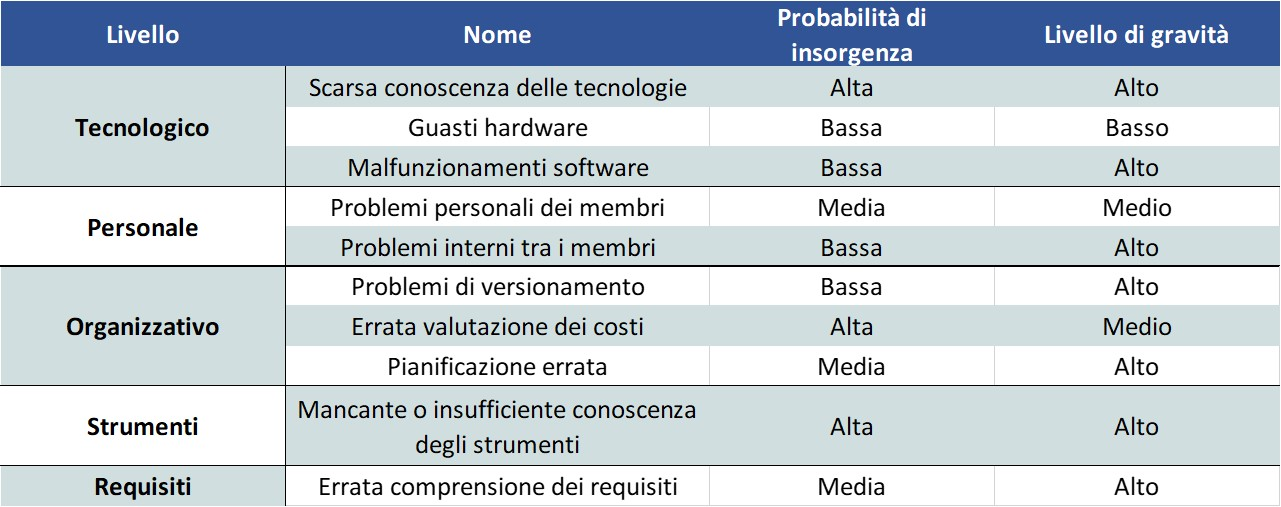
\includegraphics[scale=0.50]{img/TabellaRischi.jpg}}
	\caption{Tabella dei rischi}
	\label{fig:tab_risc}
\end{figure}


\subsection{Livello tecnologico}
\subsubsection{Scarsa conoscenza delle tecnologie}

\paragraph {Identificazione}
Alcune delle tecnologie utilizzate sono sconosciute a uno o più membri del gruppo, mentre altre sono state viste solo in ambito teorico. In generale, esistono tecnologie con cui il gruppo non ha il grado di dimestichezza richiesto.

\paragraph {Analisi}
\begin{itemize}
	\item \textbf{Probabilità di insorgenza:} Alta.
	\item \textbf{Livello di rischio:} Alto.
	\item \textbf{Possibili conseguenze:} ritardi nei tempi prestabiliti, un maggiore numero di errori.
\end{itemize}

\paragraph {Pianificazione}
I membri del gruppo si impegnano a documentarsi in modo autonomo e responsabile. Saranno seguiti dagli \adms{}, che forniranno le documentazioni necessarie e si cercherà di condividere il più possibile le conoscenze di ognuno dei membri del gruppo.

\paragraph {Contenimento} Nel caso in cui dovessero comunque presentarsi problemi, il \RdP{} provvederà a sollevare momentaneamente il membro carente dal proprio incarico per permettergli di aggiornarsi nel minor tempo possibile. 

\subsubsection{Guasti hardware}
\paragraph {Identificazione}
Viene tenuto conto di possibili guasti dei dispositivi utilizzati per lavorare dei membri del gruppo. Si includono possibili malfunzionamenti di PC e problemi alla linea internet.

\paragraph {Analisi}
\begin{itemize}
	\item \textbf{Probabilità di insorgenza:} Bassa.
	\item \textbf{Livello di rischio:} Basso.
	\item \textbf{Possibili conseguenze:} ritardi nei tempi prestabiliti, possibile perdita del lavoro temporaneo svolto.
\end{itemize}

\paragraph {Pianificazione}
Per evitare perdite di dati significativi, i membri del gruppo eseguiranno backup regolari su \emph{repository}\ped{G}. In caso di guasti i componenti del gruppo si impegnano a proseguire il proprio lavoro tramite un altro dispositivo personale o uno presente nelle aule informatiche dell'università.

\paragraph {Contenimento}
Se dovessero insorgere dei problemi si provvederà a recuperare la versione aggiornata del materiale da repository.	Il membro interessato potrà utilizzare gli altri dispositivi sopracitati nel tempo necessario alla riparazione/sostituzione.

\subsubsection{Malfunzionamenti software}
\paragraph {Identificazione}
È possibile che, nel corso del progetto, i software utilizzati incorrano in dei malfunzionamenti che potrebbero causare perdita di dati o incompatibilità tra versioni in possesso di membri diversi.

\paragraph {Analisi}
\begin{itemize}
	\item \textbf{Probabilità di insorgenza:} Bassa.
	\item \textbf{Livello di rischio:} Alto.
	\item \textbf{Possibili conseguenze:} ritardi nei tempi prestabiliti, impossibilità o ritardi per un membro di completare il proprio compito, possibile perdita di dati significativi.
\end{itemize}

\paragraph {Pianificazione}
Oltre alle strategie di backup già illustrate precedentemente, gli \adms{} si impegnano a garantire che tutti i membri del gruppo dispongano della stessa versione del software.

\paragraph {Contenimento}
Qualora un membro dovesse rilevare problemi software provvederà a comunicarlo tempestivamente agli \adms{}; qualora il problema riguardasse invece l'intero gruppo, spetterà al \RdP{} decidere se cambiare software o utilizzarne un'altra versione, previo consulto con gli \adms{}.

\subsection{Livello personale}
\subsubsection{Problemi personali dei membri}
\paragraph {Identificazione}
Vengono presi in considerazione gli eventi imprevisti che potrebbero influire sulla disponibilità dei membri del gruppo, come per esempio periodi di malattia o complicazioni famigliari.

\paragraph {Analisi}
\begin{itemize}
	\item \textbf{Probabilità di insorgenza:} Media.
	\item \textbf{Livello di rischio:} Medio.
	\item \textbf{Possibili conseguenze:} ritardi nei tempi prestabiliti.
\end{itemize}

\paragraph {Pianificazione}
I membri del gruppo, sfruttando i canali di comunicazione predisposti, provvederanno ad informare tempestivamente i propri colleghi. Nel caso in cui l'indisponibilità del componente si prolungasse, il \RdP{} provvederà a ridurre il carico lavorativo e a modificare la pianificazione. Per arginare questo rischio sono stati previsti, ove possibile, dei periodi di slack.

\paragraph {Contenimento}
Qualora dovessero insorgere problemi, il \RdP{} ripartirà il lavoro, andando a sfruttare, se necessario, i periodi di slack prestabiliti. 

\subsubsection{Problemi interni tra i membri}
\paragraph {Identificazione}
Per ogni componente del gruppo è la prima esperienza di lavoro in un gruppo di grandi dimensioni. Tale fattore potrebbe causare problemi di collaborazione causando squilibri interni, provocando così dei ritardi nei lavori ed un clima non proficuo.

\paragraph {Analisi}
\begin{itemize}
	\item \textbf{Probabilità di insorgenza:} Bassa.
	\item \textbf{Livello di rischio:} Alto.
	\item \textbf{Possibili conseguenze:} ritardi nei tempi prestabiliti, blocco delle attività, peggioramento dell'ambiente lavorativo.
\end{itemize}

\paragraph {Pianificazione}
I membri del gruppo si impegnano a tenere un atteggiamento responsabile e maturo, andando subito a esternare eventuali dissapori tra loro e conferendo con il \RdP{} quando non riescano a gestire le loro incompatibilità.

\paragraph {Contenimento}
Se dovessero sorgere problemi per cui sia necessario l'intervento del \RdP{}, questi cercherà di appianare le divergenze e, se necessario, provvederà a riorganizzare il lavoro, separando i membri coinvolti.

\subsection{Livello organizzativo}
\subsubsection{Problemi di versionamento}
\paragraph {Identificazione}
Poiché i membri del gruppo non hanno mai lavorato prima a progetti così complessi e che richiedessero coordinazione tra tante persone, esiste la possibilità che si creino problemi di versionamento quando più persone sono incaricate di redigere o verificare lo stesso documento o la stessa parte di codice.

\paragraph {Analisi}
\begin{itemize}
	\item \textbf{Probabilità di insorgenza:} Bassa.
	\item \textbf{Livello di rischio:} Alto.
	\item \textbf{Possibili conseguenze:} ritardi nei tempi prestabiliti, confusione ed errori.
\end{itemize}

\paragraph {Pianificazione}
È stato predisposto un \emph{tracker}\ped{G} in modo che ogni cambiamento sia sempre notificato e controllato. Il \RdP{} fornisce una divisione di ruoli che i membri si impegnano a seguire senza accavallarsi.

\paragraph {Contenimento}
In caso di problemi si provvederà e recuperare l'ultima versione corretta da repository.

\subsubsection{Errata valutazione dei costi}
\paragraph {Identificazione}
Poiché i membri del gruppo non hanno esperienze precedenti, è possibile che, nella fase di pianificazione, vengano sottostimati i costi, non solo economici, ma anche in termini di tempo.

\paragraph {Analisi}
\begin{itemize}
	\item \textbf{Probabilità di insorgenza:} Alta.
	\item \textbf{Livello di rischio:} Medio.
	\item \textbf{Possibili conseguenze:} ritardi nei tempi prestabiliti.
\end{itemize}

\paragraph {Pianificazione}
Il \RdP{} terrà sempre sotto controllo lo stato di avanzamento delle varie fasi rispetto alla pianificazione iniziale. Dove possibile andrà a sfruttare i periodi di slack predisposti, eventualmente ripianificando il lavoro del gruppo.

\paragraph {Contenimento}
In caso di ritardi il lavoro verrà ripianificato, cercando di rientrare nei tempi stabiliti.

\subsubsection{Pianificazione errata}
\paragraph {Identificazione}
Durante la pianificazione è possibile che i tempi per l'esecuzione di alcune attività vengano calcolati in modo errato.

\paragraph {Analisi}
\begin{itemize}
	\item \textbf{Probabilità di insorgenza:} Media.
	\item \textbf{Livello di rischio:} Alto.
	\item \textbf{Possibili conseguenze:} ritardi nei tempi prestabiliti.
\end{itemize}

\paragraph {Pianificazione}
La caratteristica dinamica del rischio impone che si debba controllare lo stato delle attività periodicamente, in modo da accertarsi dell'avanzamento previsto nello svolgimento dei vari task e verificare eventuali ritardi nello sviluppo di questi.

\paragraph {Contenimento}
Per ogni attività, il \RdP{}, prevederà un periodo maggiore di quanto normalmente richiesto, in modo tale che un eventuale ritardo non influenzi la durata totale del progetto.

\subsection{Strumenti}
\subsubsection{Mancante o insufficiente conoscenza degli strumenti}
\paragraph {Identificazione}
Lo sviluppo del progetto richiede l'utilizzo di vari strumenti mai utilizzati prima dal gruppo o il cui uso non è stato esaustivo.

\paragraph{Analisi}
\begin{itemize}
	\item \textbf{Probabilità di insorgenza:} Alta.
	\item \textbf{Livello di rischio:} Alto.
	\item \textbf{Possibili conseguenze:} ritardi nei tempi prestabiliti, rallentamenti nelle varie attività.
\end{itemize}

\paragraph {Pianificazione}

Ogni volta che sarà ritenuto necessario, dal \RdP{} e dagli \adms{}, utilizzare un nuovo strumento, tutti i membri del gruppo verranno subito avvertiti. L'introduzione di nuovi strumenti sarà sempre una scelta pesata e responsabile, consapevole degli alti livelli di rischio che può comportare. \\
Una volta introdotto tale strumento, il gruppo si dovrà documentare su come impiegarlo al meglio seguendo le indicazioni fornite dall’\adm{}.

\paragraph {Contenimento}
Se tutti i membri del gruppo dovessero riscontrare gravi difficoltà nell'apprendimento di uno strumento, o se il \RdP{} riterrà i tempi di apprendimento troppo lunghi, si opterà per la selezione di un altro strumento più adatto.

\subsection{Requisiti}
\subsubsection{Errata comprensione dei requisiti}
\paragraph{Identificazione}
Si preventiva una mancata comprensione tra il gruppo e il proponente, che può portare a inesattezze nei requisiti e nella comprensione del prodotto che il proponente e il committente si aspettano.

\paragraph{Analisi}
\begin{itemize}
	\item \textbf{Probabilità di insorgenza:} Media.
	\item \textbf{Livello di rischio:} Alto.
	\item \textbf{Possibili conseguenze:} ritardi nei tempi prestabiliti, rallentamenti nelle varie fasi, possibilità di dover tornare sui propri passi.
\end{itemize}

\paragraph {Pianificazione}
Si è cercato di ridurre al minimo la possibilità di insorgenza di questo rischio confrontandosi col proponente e col committente. Soprattutto nel periodo di \AdR{}, si vuole rendere il proponente partecipe, chiedendo spesso il suo parere ed il suo feedback.

\paragraph {Contenimento}
Per ogni dubbio, sarà necessario un confronto con il proponente in modo da poter definire con chiarezza ogni requisito necessario al corretto sviluppo del progetto. Sarà inoltre indispensabile correggere eventuali errori o imprecisioni indicati dal committente all’esito di ogni revisione.
%\newpage
\section{Pianificazione}

Per migliorare lo sviluppo del progetto e rispettare le scadenze elencate al punto \hyperref[Scadenze]{1.6} di questo documento, lo sviluppo è stato suddiviso in sei periodi, ripartiti a loro volta in due macro periodi indicanti il primo, un periodo di investimento a carico del gruppo \Gruppo{} ed il secondo, facente parte del preventivo a carico dell'azienda proponente.

Periodo di investimento:
\begin{itemize}
\item \textbf{Analisi dei requisiti};
\item \textbf{Analisi dei requisiti in dettaglio}.
\end{itemize}
Periodo rendicontabile:
\begin{itemize}
\item \textbf{Prototipazione};
\item \textbf{Prototipazione in dettaglio};
\item \textbf{Progettazione finale e Codifica};
\item \textbf{Codifica in dettaglio, Validazione e Collaudo}.
\end{itemize}
Di seguito sono analizzati in dettaglio i periodi sopracitati e per ognuno di essi viene riportato il diagramma di Gantt; il diagramma riporta le milestone e le date di inizio e fine di ciascuna attività.

\subsection{Analisi dei requisiti}
\textbf{Periodo}: dal 2018-03-03 al 2018-04-13 (RR)\\

Questo periodo comincia con la creazione del gruppo e si conclude con la consegna dei documenti per accedere alla \RR{}.\\
I documenti stilati e successivamente verificati durante questo periodo sono:
\begin{itemize}
\item \textbf{Norme di Progetto}: questo è il primo documento redatto in ordine cronologico poiché norma lo svolgimento di tutte le attività del gruppo \Gruppo{}; esso è indipendente dal capitolato scelto;
\item \textbf{Studio di fattibilità}: in questo documento vengono analizzati tutti i capitolati proposti. Per ognuno viene analizzato il dominio applicativo e tecnologico, valutandone i fattori positivi e negativi. È un’attività critica perché definisce il progetto sul quale il gruppo andrà a lavorare e blocca la stesura del documento di \AdR{};
\item \textbf{Piano di Progetto}: vengono pianificate tutte le attività necessarie allo svolgimento del progetto ed assegnate alle risorse disponibili, distribuendo il carico di lavoro in maniera uniforme;
\item \textbf{Piano di Qualifica}: vengono definiti gli standard qualitativi e le metriche da utilizzare per verifica e validazione;
\item \textbf{Analisi dei Requisiti}: viene effettuata l’analisi approfondita del capitolato scelto con lo \SdF{} e vengono identificati i requisiti obbligatori e facoltativi;
\item \textbf{Glossario}: contiene la definizione di alcuni termini utilizzati nei vari documenti, al fine di eliminare ogni possibile ambiguità di significato;
\item \textbf{Lettera di Presentazione}: documento che dichiara l’interesse del gruppo a partecipare alla gara d’appalto.
\end{itemize}

\begin{figure}[h!]
	\centerline{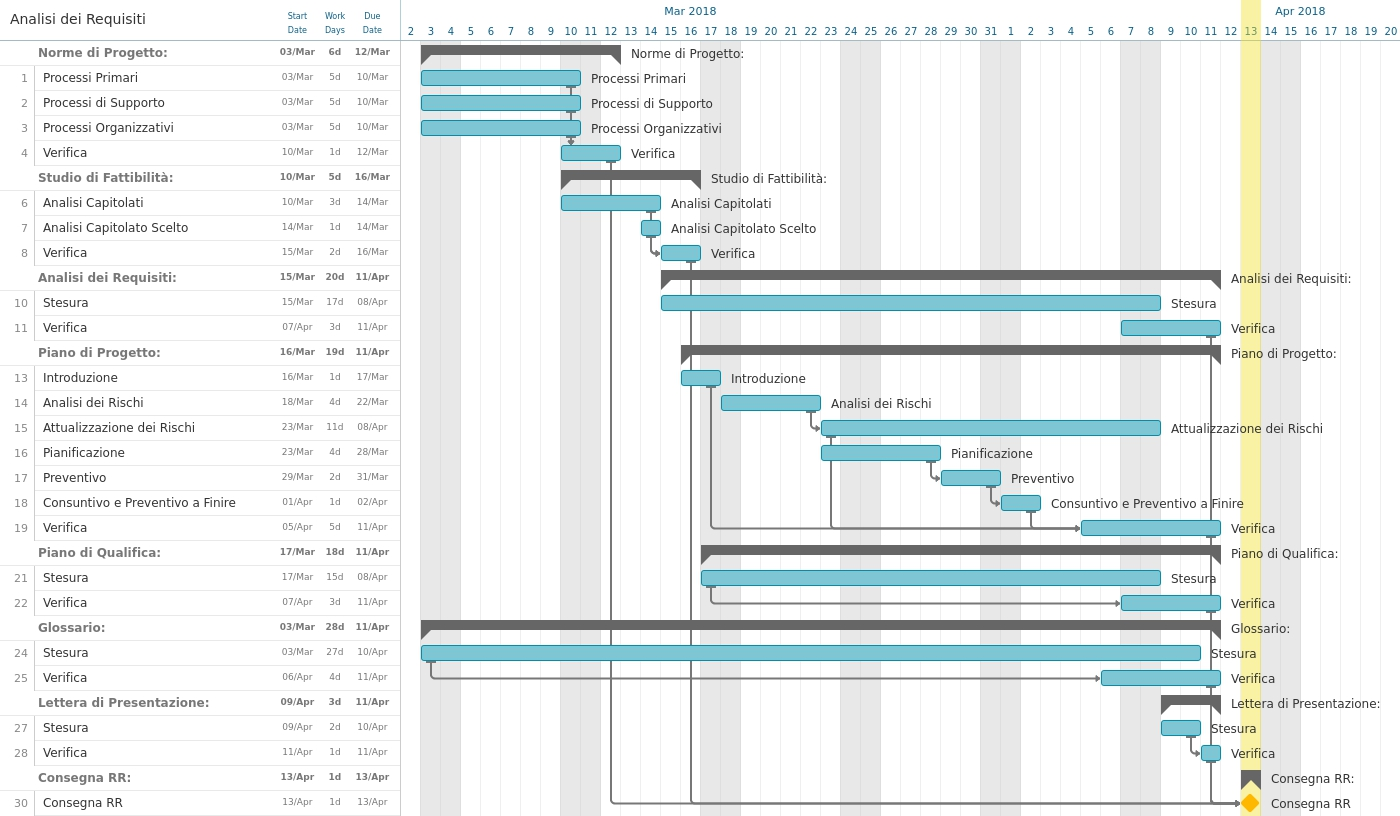
\includegraphics[scale=0.35]{img/DiagrammiGantt/AnalisiRequisiti.jpg}}
	\caption{Diagramma di Gantt: Analisi dei requisiti}
	\label{fig:gantt_ana_req}
\end{figure}
\clearpage

\subsection{Analisi dei Requisiti in dettaglio}
\textbf{Periodo}: dal 2018-04-14 (RR) al 2018-04-26 (Milestone Interna)\\

In attesa dell'esito della \RR{}, i membri del gruppo si impegnano a colmare le proprie lacune tecnologiche necessarie allo svolgimento del progetto. Parallelamente, si mira a consolidare ed ampliare i requisiti richiesti dal sistema e a migliorare il documento di \AdR{} attuando le correzioni in base all’esito della \RR{}; vengono inoltre corretti e verificati anche gli altri documenti. Il termine fissato per la conclusione di questa fase corrisponde ad una milestone interna.

\begin{figure}[h!]
	\centerline{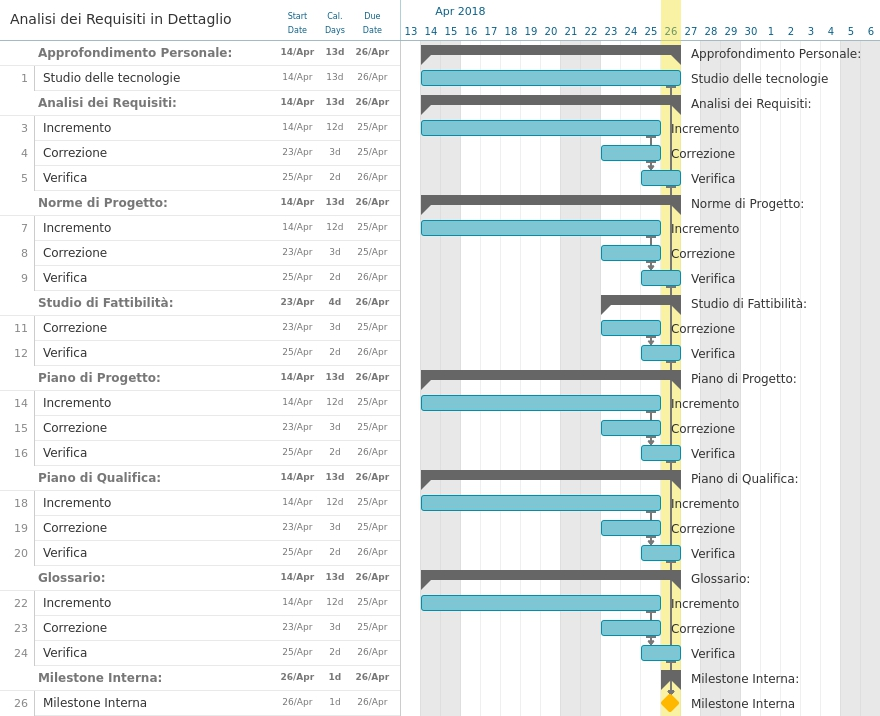
\includegraphics[scale=0.55]{img/DiagrammiGantt/AnalisiRequisitiDettaglio.jpg}}
	\caption{Diagramma di Gantt: Analisi dei requisiti in Dettaglio}
	\label{fig:gantt_ana_req_dett}
\end{figure}
\clearpage

\subsection{Prototipazione}
\textbf{Periodo}: dal 2018-04-27 (Milestone Interna) al 2018-05-07 (RP)\\

Questo periodo è caratterizzato dalla realizzazione di un prototipo utilizzando le tecnologie necessarie, sulla base delle scelte del gruppo \Gruppo{} e delle richieste del proponente.
Lo scopo è quello di comprendere pienamente il dominio tecnologico del progetto e realizzare i casi d'uso ritenuti più importanti e significativi per la buona riuscita del prodotto finale, realizzando così una \emph{Technology Baseline}\ped{G}. \\ 
Come attività di supporto si incrementano i documenti già redatti nei periodi precedenti.\\
Per semplicità si considera come periodo di consegna e presentazione della Technology Baseline la data di \RP{}; sarà poi specificata una scadenza più precisa in fase di sviluppo.

\begin{figure}[h!]
	\centerline{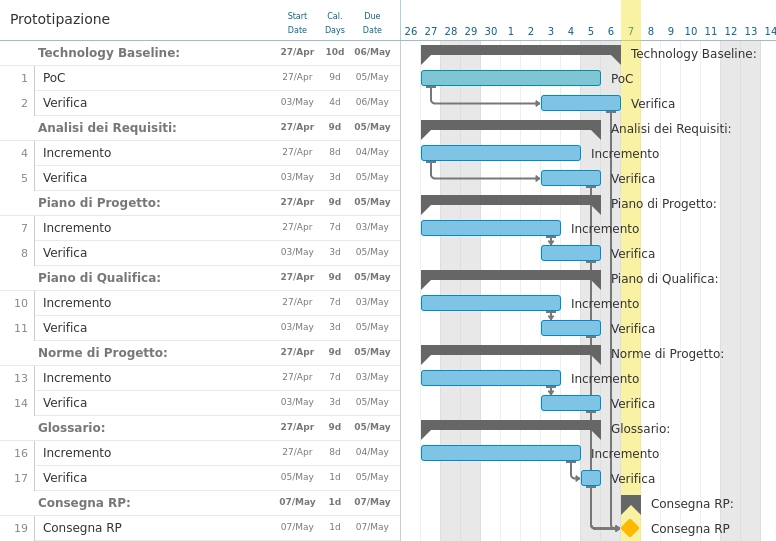
\includegraphics[scale=0.55]{img/DiagrammiGantt/Prototipazione.jpg}}
	\caption{Diagramma di Gantt: Prototipazione}
	\label{fig:gantt_prot}
\end{figure}
\clearpage

\subsection{Prototipazione in Dettaglio}
\textbf{Periodo}: dal 2018-05-08 (RP) al 2018-05-16 (Milestone Interna)\\

In attesa dell'esito della \RP{}, si incrementa la \emph{PoC}\ped{G} finora realizzata, migliorando i requisiti già interessati. In seguito verranno effettuate le dovute correzioni a questa e ai documenti in base all'esito della \RP{}. La conclusione di questo periodo corrisponde ad una milestone interna.

\begin{figure}[h!]
	\centerline{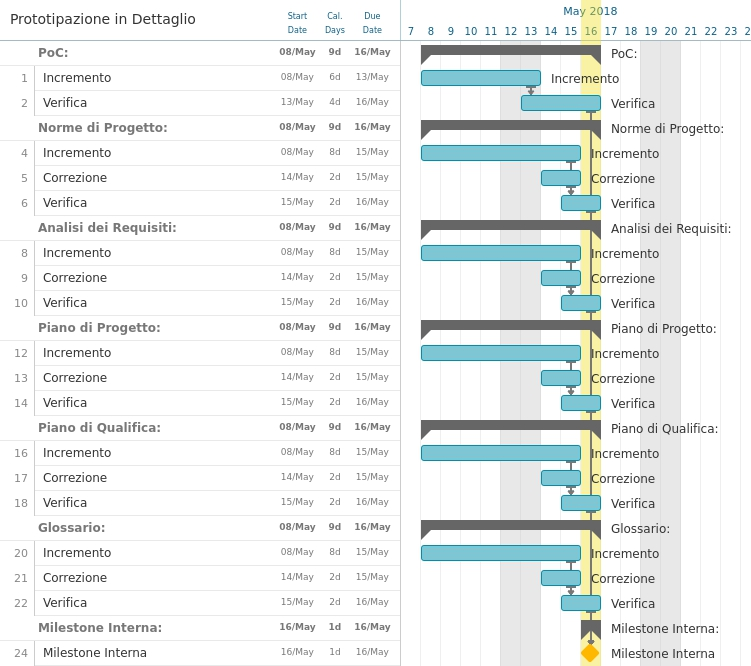
\includegraphics[scale=0.55]{img/DiagrammiGantt/PrototipazioneDettaglio.jpg}}
	\caption{Diagramma di Gantt: Prototipazione in dettaglio}
	\label{fig:gantt_prot_dett}
\end{figure}
\clearpage

\subsection{Progettazione finale e Codifica}
\textbf{Periodo}: dal 2018-05-17 (Milestone Interna) al 2018-06-08 (RQ)\\

Si procede con la progettazione in dettaglio dell'architettura di sistema, comprensiva di design pattern implementati e diagrammi delle classi e di sequenza; il risultato di questo insieme di attività comporrà la \emph{ProductBaseline}\ped{G} del prodotto. Una volta definita, si procede con la fase di codifica per realizzare i requisiti obbligatori stabiliti in precedenza, riutilizzando ed ampliando il codice prodotto durante la fase di Prototipazione e Prototipazione in Dettaglio. \\
Come attività di supporto si incrementano alcuni documenti già redatti nei periodi precedenti e si stilano due nuovi documenti:
\begin{itemize}
	\item \textbf{Manuale Utente}: contiene indicazioni utili all'utente finale per l'utilizzo del prodotto
	\item \textbf{Manuale Sviluppatore}: contiene indicazioni utili allo sviluppatore per la manutenzione e l'incremento del prodotto
\end{itemize}
Per semplicità si considera come periodo di consegna e presentazione della Product Baseline la data di \RQ{}; sarà poi specificata una scadenza più precisa in fase di sviluppo.

\begin{figure}[h!]
	\centerline{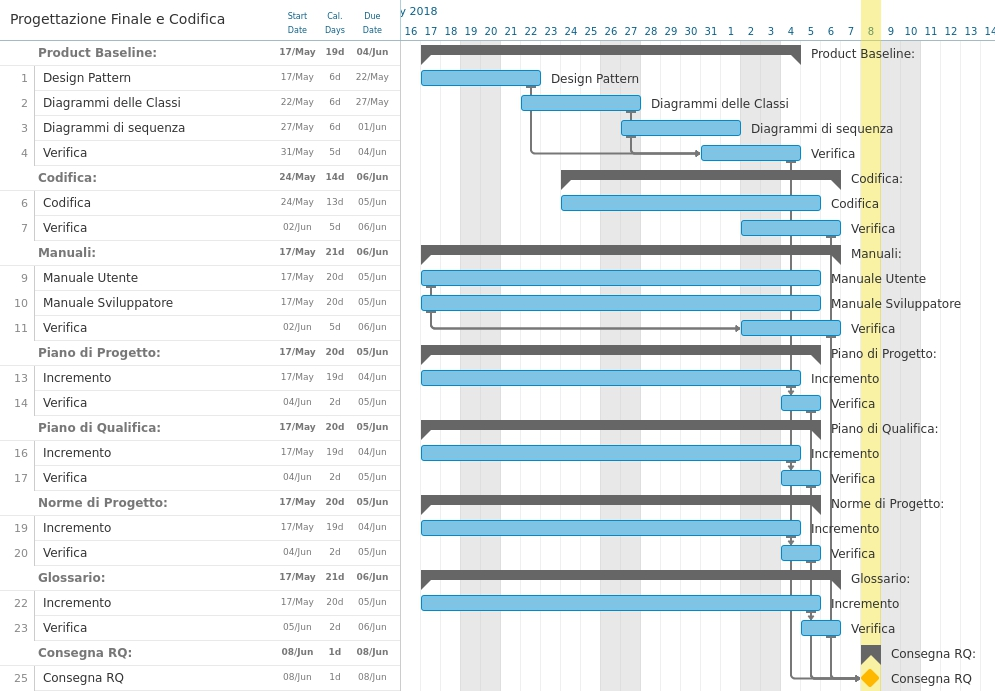
\includegraphics[scale=0.5]{img/DiagrammiGantt/ProgettazioneFinaleCodifica.jpg}}
	\caption{Diagramma di Gantt: Progettazione finale e Codifica}
	\label{fig:gantt_prog_fin_cod}
\end{figure}
\clearpage

\subsection{Codifica in Dettaglio, Validazione e Collaudo}
\textbf{Periodo}: dal 2018-06-15 (RQ) al 2018-07-15 (RA)\\

Durante quest'ultimo periodo di sviluppo, si incrementano i documenti redatti finora e si effettuano gli ultimi incrementi di codifica; a seguito di queste attività si procede con la verifica del sistema completo e il collaudo di esso.

\begin{figure}[h!]
	\centerline{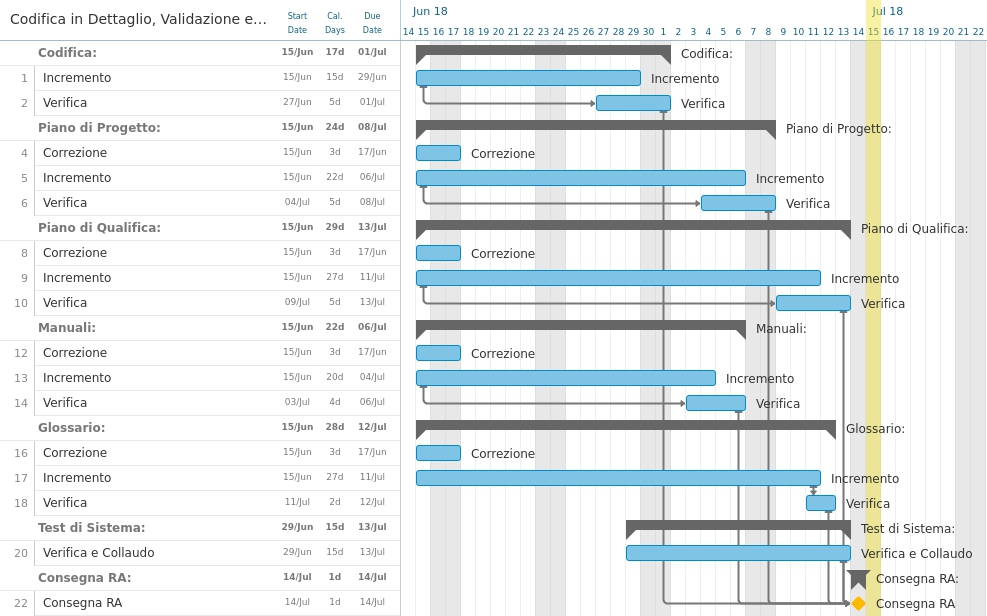
\includegraphics[scale=0.45]{img/DiagrammiGantt/CodificaValidazioneCollaudo.jpg}}
	\caption{Diagramma di Gantt: Codifica in dettaglio, Validazione e Collaudo}
	\label{fig:gantt_cod_valid_coll}
\end{figure}
\clearpage

%\newpage
\section{Preventivo}

Viene di seguito riportato il preventivo per il \NomeProgetto{}; esso si divide, per ogni periodo, in:
\begin{itemize}
	\item \textbf{Prospetto orario}: presenta la distribuzione oraria e la suddivisione nei ruoli per ogni membro del gruppo \gruppo;
	\item \textbf{Prospetto economico}: presenta le ore di impegno calcolate per i ruoli coinvolti ed il rispettivo costo.
\end{itemize}
La suddivisione oraria viene fatta tenendo conto delle seguenti regole:
\begin{itemize}
	\item Ogni membro del gruppo dovrà sostenere una mole di lavoro comparabile, quindi il totale delle ore dovrà essere equamente distribuito tra i membri;
	\item Ogni membro del gruppo dovrà ricoprire ogni ruolo almeno una volta durante il ciclo di sviluppo del prodotto;
	\item In nessun caso si dovrà verificare un conflitto di interessi in cui un \ver{} debba	controllare il proprio lavoro.
\end{itemize}
Le sigle utilizzate per i vari ruoli saranno:
\begin{itemize}
	\item \textbf{Re}: \RdP;
	\item \textbf{Ad}: \adm;
	\item \textbf{An}: \ana;
	\item \textbf{Pr}: \prog;
	\item \textbf{Pg}: \progr;
	\item \textbf{Ve}: \ver.
\end{itemize}
Per il preventivo si tiene conto che i primi due periodi sono considerati di investimento del gruppo e non a carico del committente, per cui le ore di impegno svolte durante questi non saranno conteggiate nelle ore totali da retribuire.
\newpage
\subsection{Attività di investimento del gruppo}
\subsubsection{Analisi dei requisiti}
\paragraph{Prospetto orario}
Il prospetto orario per questo periodo è illustrato in tabella.
\begin{table}[H]
	\centerline{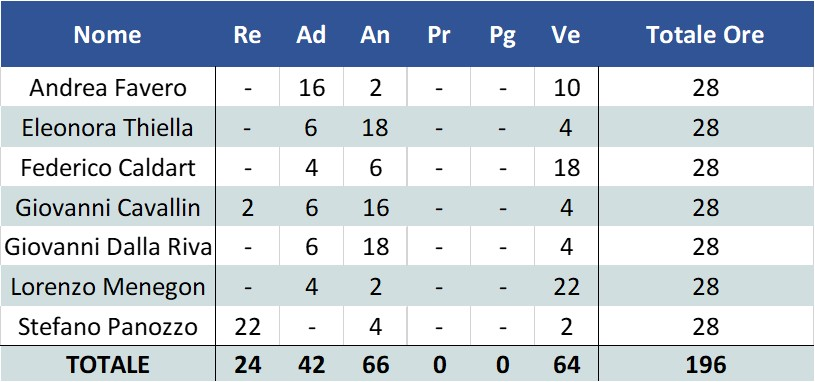
\includegraphics[scale=0.7]{img/Preventivo/AnalisiRequisitiOrario.jpg}}
	\caption{Prospetto Orario: Analisi dei requisiti}
	\clearpage
\end{table}
La raffigurazione grafica della suddivisione dei ruoli all'interno del gruppo è così rappresentata: 
\begin{figure}[H]
	\centerline{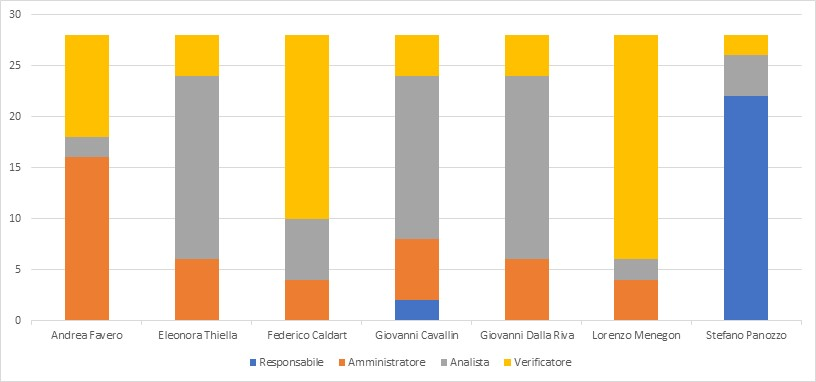
\includegraphics[scale=0.85]{img/Preventivo/Istogrammi/AnalisiRequisiti.jpg}}
	\caption{Raffigurazione Prospetto Orario: Analisi dei requisiti}
	\clearpage
\end{figure}
\newpage
\paragraph{Prospetto economico}
Il prospetto economico per questo periodo è illustrato in tabella. Notare che le spese per questa attività non sono a carico del committente.
\begin{table}[H]
	\centerline{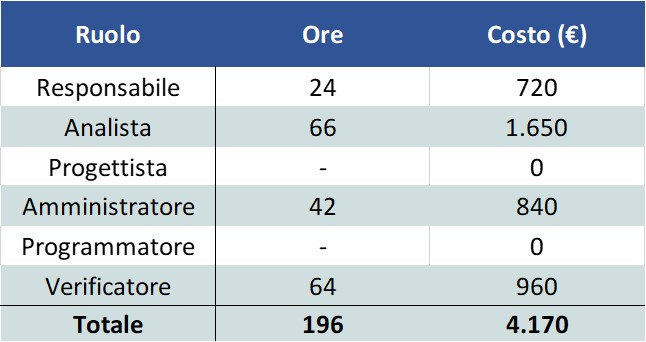
\includegraphics[scale=0.7]{img/Preventivo/AnalisiRequisitiEconomico.jpg}}
	\caption{Prospetto Economico: Analisi dei requisiti}
	\clearpage
\end{table}
La raffigurazione grafica del peso di ogni ruolo sul costo totale è così rappresentata: 
\begin{figure}[H]
	\centerline{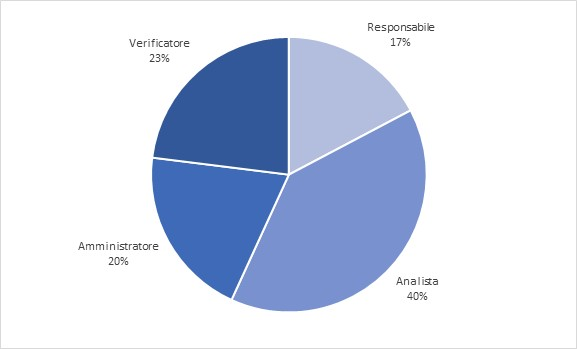
\includegraphics[scale=0.9]{img/Preventivo/Torte/AnalisiRequisiti.jpg}}
	\caption{Raffigurazione Prospetto Economico: Analisi dei requisiti}
	\clearpage
\end{figure}
\newpage
\subsubsection{Analisi dei requisiti in dettaglio}
\paragraph{Prospetto orario}
Il prospetto orario per questo periodo è illustrato in tabella.
\begin{table}[H]
	\centerline{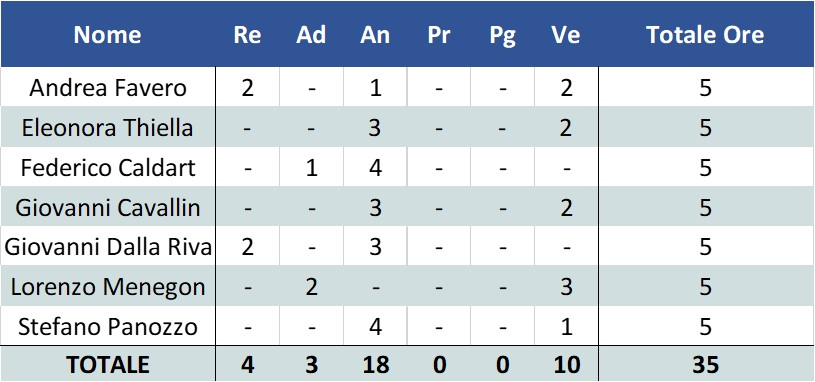
\includegraphics[scale=0.7]{img/Preventivo/AnalisiRequisitiDettaglioOrario.jpg}}
	\caption{Prospetto Orario: Analisi dei requisiti in dettaglio}
	\clearpage
\end{table}
La raffigurazione grafica della suddivisione dei ruoli all'interno del gruppo è così rappresentata: 
\begin{figure}[H]
	\centerline{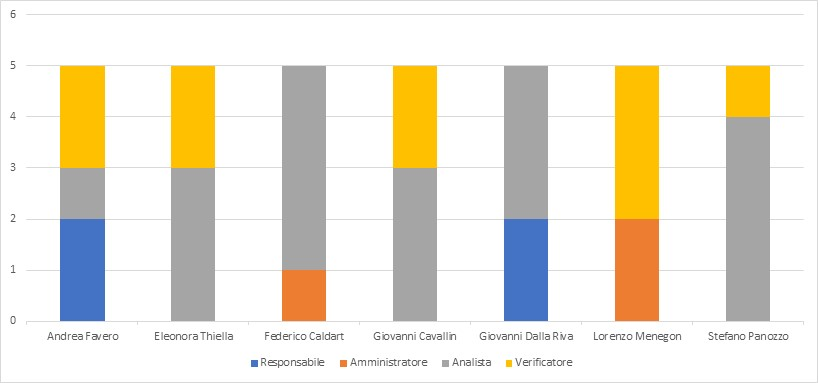
\includegraphics[scale=0.85]{img/Preventivo/Istogrammi/AnalisiRequisitiDettaglio.jpg}}
	\caption{Raffigurazione Prospetto Orario: Analisi dei requisiti in dettaglio}
	\clearpage
\end{figure}
\newpage
\paragraph{Prospetto economico}
Il prospetto economico per questo periodo è illustrato in tabella. Notare che le spese per questa attività non sono a carico del committente.
\begin{table}[H]
	\centerline{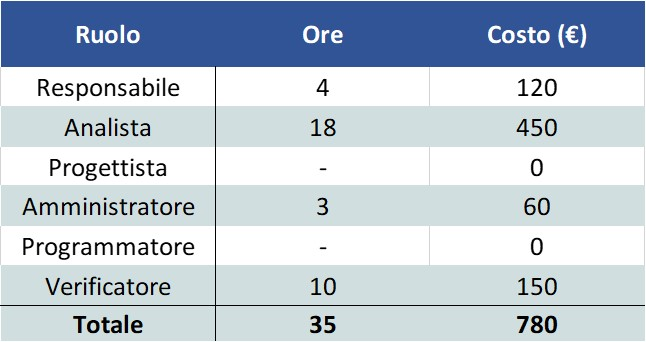
\includegraphics[scale=0.7]{img/Preventivo/AnalisiRequisitiDettaglioEconomico.jpg}}
	\caption{Prospetto Economico: Analisi dei requisiti in dettaglio}
	\clearpage
\end{table}
La raffigurazione grafica del peso di ogni ruolo sul costo totale è così rappresentata: 
\begin{figure}[H]
	\centerline{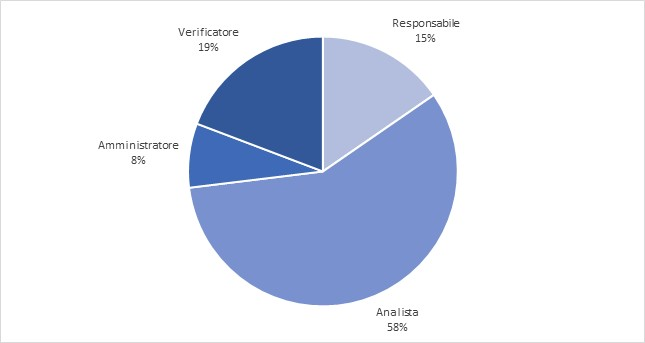
\includegraphics[scale=0.9]{img/Preventivo/Torte/AnalisiRequisitiDettaglio.jpg}}
	\caption{Raffigurazione Prospetto Economico: Analisi dei requisiti in dettaglio}
	\clearpage
\end{figure}
\newpage
\subsection{Attività a carico del committente}
\subsubsection{Prototipazione}
\paragraph{Prospetto orario}
Il prospetto orario per questo periodo è illustrato in tabella.
\begin{table}[H]
	\centerline{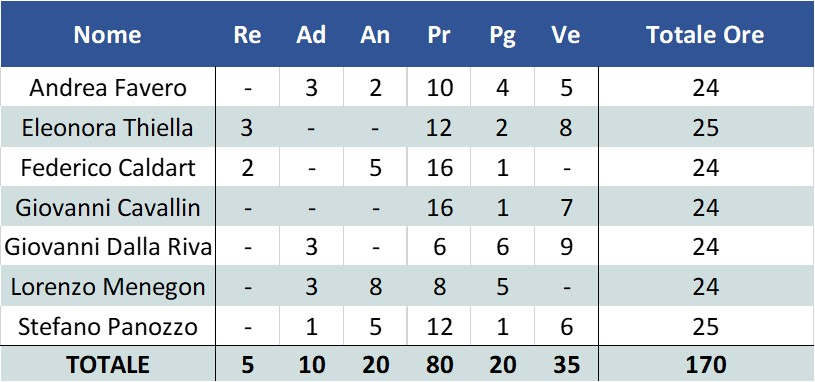
\includegraphics[scale=0.7]{img/Preventivo/PrototipazioneOrario.jpg}}
	\caption{Prospetto Orario: Prototipazione}
	\clearpage
\end{table}
La raffigurazione grafica della suddivisione dei ruoli all'interno del gruppo è così rappresentata: 
\begin{figure}[H]
	\centerline{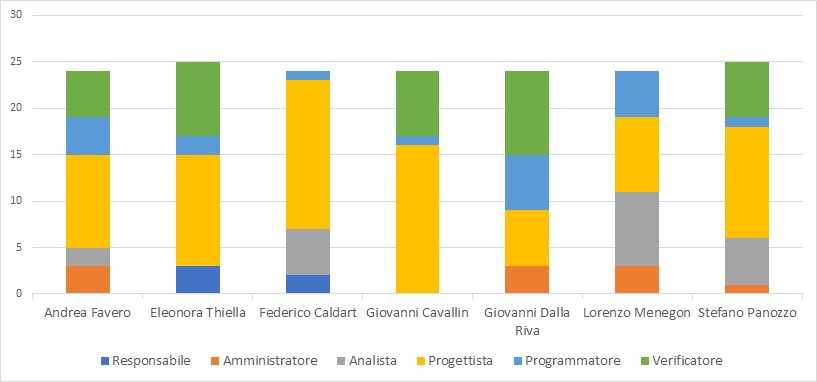
\includegraphics[scale=0.85]{img/Preventivo/Istogrammi/Prototipazione.jpg}}
	\caption{Raffigurazione Prospetto Orario: Prototipazione}
	\clearpage
\end{figure}
\newpage
\paragraph{Prospetto economico}
Il prospetto economico per questo periodo è illustrato in tabella. 
\begin{table}[H]
	\centerline{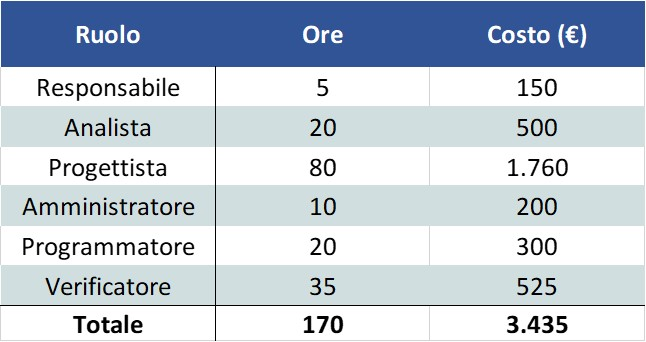
\includegraphics[scale=0.7]{img/Preventivo/PrototipazioneEconomico.jpg}}
	\caption{Prospetto Economico: Prototipazione}
	\clearpage
\end{table}
La raffigurazione grafica del peso di ogni ruolo sul costo totale è così rappresentata: 
\begin{figure}[H]
	\centerline{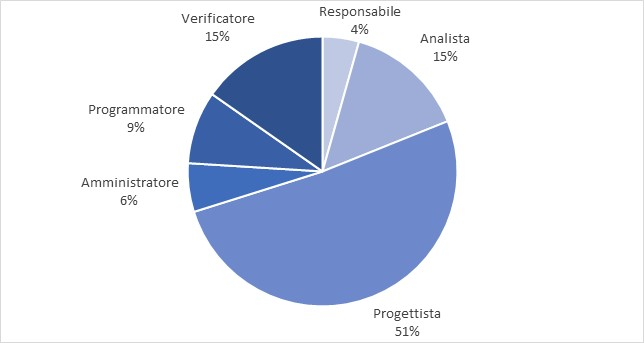
\includegraphics[scale=0.9]{img/Preventivo/Torte/Prototipazione.jpg}}
	\caption{Raffigurazione Prospetto Economico: Prototipazione}
	\clearpage
\end{figure}
\newpage
\subsubsection{Prototipazione in dettaglio}
\paragraph{Prospetto orario}
Il prospetto orario per questo periodo è illustrato in tabella.
\begin{table}[H]
	\centerline{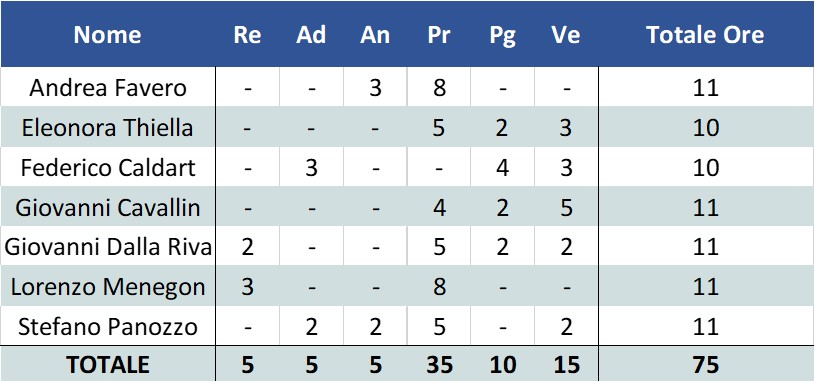
\includegraphics[scale=0.7]{img/Preventivo/PrototipazioneDettaglioOrario.jpg}}
	\caption{Prospetto Orario: Prototipazione in dettaglio}
	\clearpage
\end{table}
La raffigurazione grafica della suddivisione dei ruoli all'interno del gruppo è così rappresentata: 
\begin{figure}[H]
	\centerline{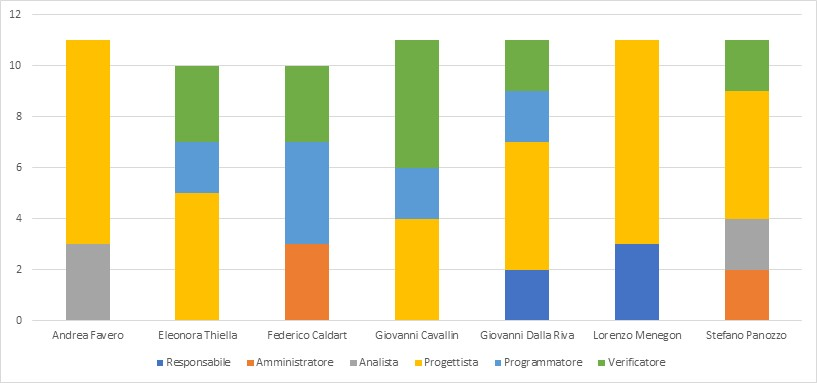
\includegraphics[scale=0.85]{img/Preventivo/Istogrammi/PrototipazioneDettaglio.jpg}}
	\caption{Raffigurazione Prospetto Orario: Prototipazione in dettaglio}
	\clearpage
\end{figure}
\newpage
\paragraph{Prospetto economico}
Il prospetto economico per questo periodo è illustrato in tabella. 
\begin{table}[H]
	\centerline{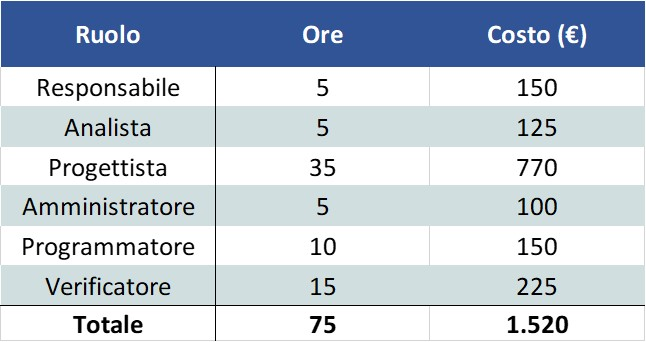
\includegraphics[scale=0.7]{img/Preventivo/PrototipazioneDettaglioEconomico.jpg}}
	\caption{Prospetto Economico: Prototipazione in dettaglio}
	\clearpage
\end{table}
La raffigurazione grafica del peso di ogni ruolo sul costo totale è così rappresentata:
\begin{figure}[H]
	\centerline{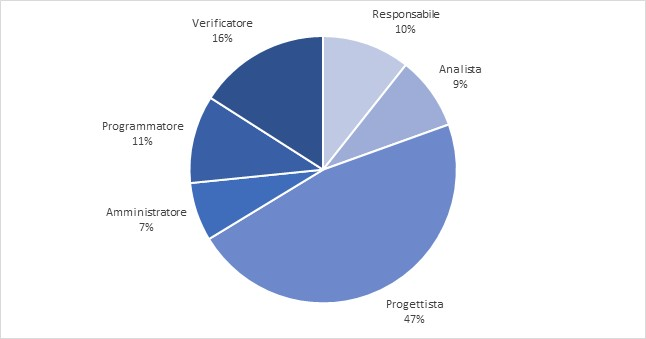
\includegraphics[scale=0.9]{img/Preventivo/Torte/PrototipazioneDettaglio.jpg}}
	\caption{Raffigurazione Prospetto Economico: Prototipazione in dettaglio}
	\clearpage
\end{figure} 
\newpage
\subsubsection{Progettazione finale e Codifica}
\paragraph{Prospetto orario}
Il prospetto orario per questo periodo è illustrato in tabella.
\begin{table}[H]
	\centerline{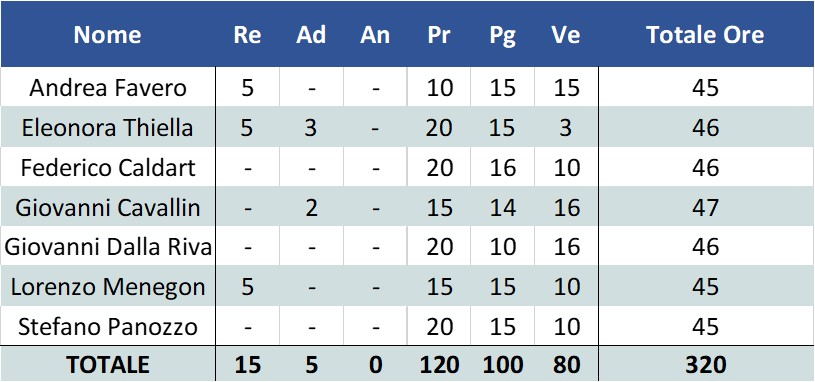
\includegraphics[scale=0.7]{img/Preventivo/ProgettazioneFinaleCodificaOrario.jpg}}
	\caption{Prospetto Orario: Progettazione finale e Codifica}
	\clearpage
\end{table}
La raffigurazione grafica della suddivisione dei ruoli all'interno del gruppo è così rappresentata: 
\begin{figure}[H]
	\centerline{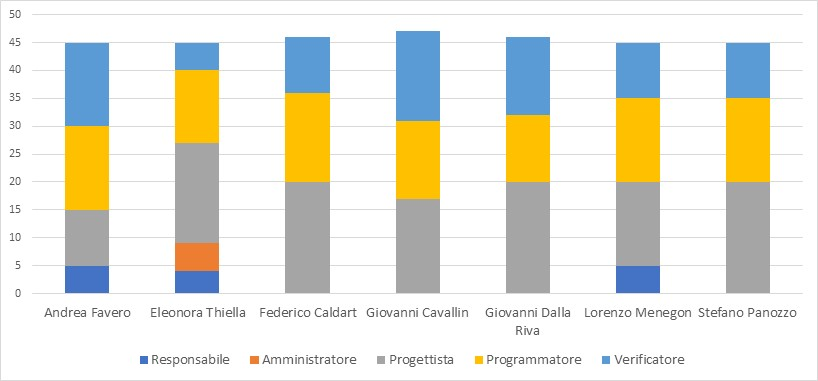
\includegraphics[scale=0.85]{img/Preventivo/Istogrammi/ProgettazioneFinaleCodifica.jpg}}
	\caption{Raffigurazione Prospetto Orario: Progettazione finale e Codifica}
	\clearpage
\end{figure}
\newpage
\paragraph{Prospetto economico}
Il prospetto economico per questo periodo è illustrato in tabella. 
\begin{table}[H]
	\centerline{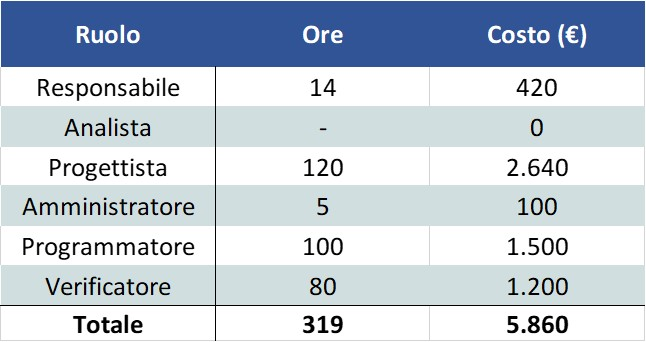
\includegraphics[scale=0.7]{img/Preventivo/ProgettazioneFinaleCodificaEconomico.jpg}}
	\caption{Prospetto Economico: Progettazione finale e Codifica}
	\clearpage
\end{table}
La raffigurazione grafica del peso di ogni ruolo sul costo totale è così rappresentata: 
\begin{figure}[H]
	\centerline{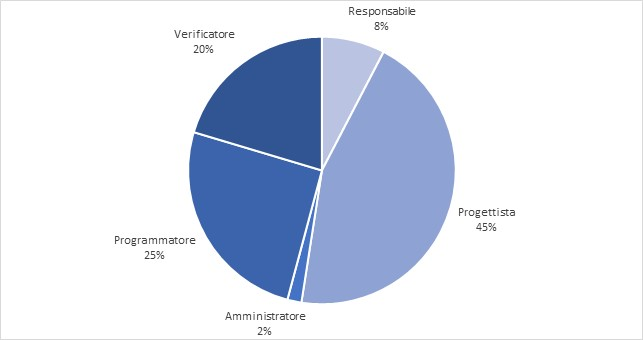
\includegraphics[scale=0.9]{img/Preventivo/Torte/ProgettazioneFinaleCodifica.jpg}}
	\caption{Raffigurazione Prospetto Economico: Progettazione finale e Codifica}
	\clearpage
\end{figure} 
\newpage
\subsubsection{Codifica in dettaglio, Validazione e Collaudo}
\paragraph{Prospetto orario}
Il prospetto orario per questo periodo è illustrato in tabella.
\begin{table}[H]
	\centerline{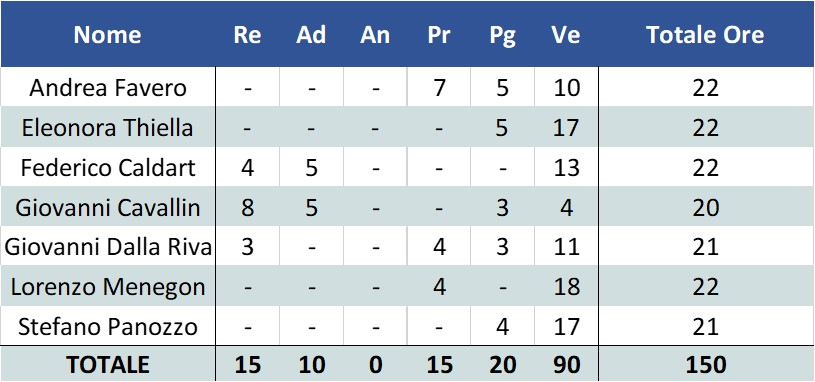
\includegraphics[scale=0.7]{img/Preventivo/CodDettaglioValidazioneCollaudoOrario.jpg}}
	\caption{Prospetto Orario: Codifica in dettaglio, Validazione e Collaudo}
	\clearpage
\end{table}
La raffigurazione grafica della suddivisione dei ruoli all'interno del gruppo è così rappresentata: 
\begin{figure}[H]
	\centerline{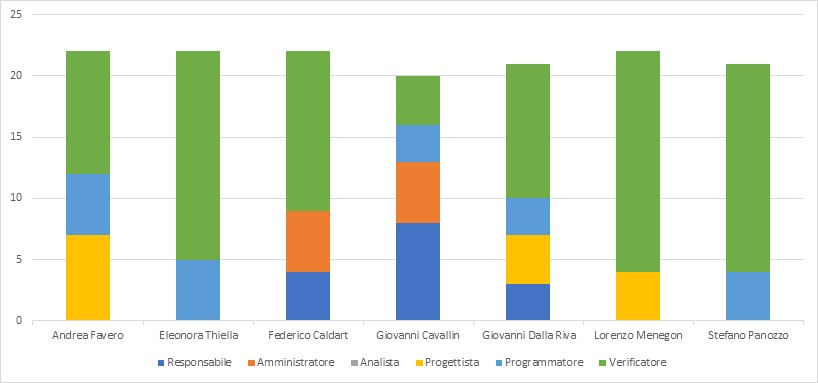
\includegraphics[scale=0.85]{img/Preventivo/Istogrammi/CodDettaglioValidazioneCollaudo.jpg}}
	\caption{Raffigurazione Prospetto Orario: Codifica in dettaglio, Validazione e Collaudo}
	\clearpage
\end{figure}
\newpage
\paragraph{Prospetto economico}
Il prospetto economico per questo periodo è illustrato in tabella. 
\begin{table}[H]
	\centerline{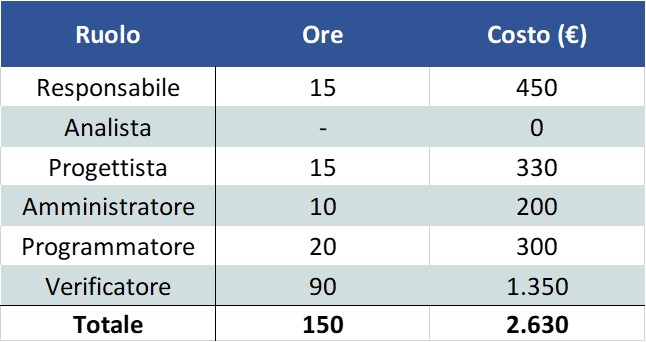
\includegraphics[scale=0.7]{img/Preventivo/CodDettaglioValidazioneCollaudoEconomico.jpg}}
	\caption{Prospetto Economico: Codifica in dettaglio, Validazione e Collaudo}
	\clearpage
\end{table}
La raffigurazione grafica del peso di ogni ruolo sul costo totale è così rappresentata: 
\begin{figure}[H]
	\centerline{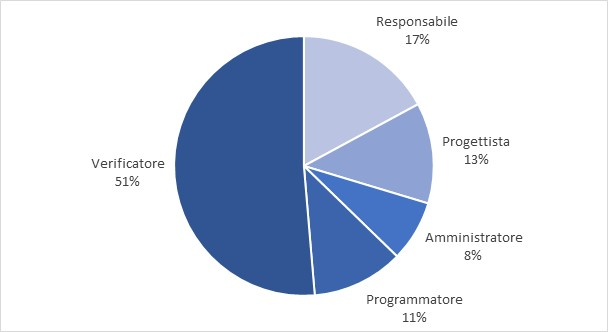
\includegraphics[scale=0.9]{img/Preventivo/Torte/CodDettaglioValidazioneCollaudo.jpg}}
	\caption{Raffigurazione Prospetto Economico: Codifica in dettaglio, Validazione e Collaudo}
	\clearpage
\end{figure} 
\newpage
\subsection{Totale}
In seguito sono presentati il prospetto orario ed economico riepilogativi per tutta la durata del progetto.\\
Si noti la differenza fra le ore totali, comprensive dell'attività di investimento iniziale a carico del gruppo, e le ore rendicontate a carico del committente.
\paragraph{Prospetto orario}
Il prospetto orario per l'intera durata del progetto è illustrato in tabella. 
\begin{table}[H]
	\centerline{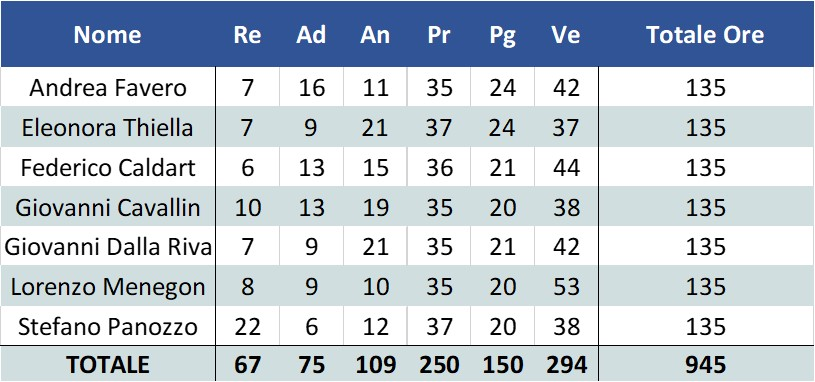
\includegraphics[scale=0.7]{img/Preventivo/TotaleOre.jpg}}
	\caption{Prospetto Orario: Riepilogo}
	\clearpage
\end{table}
La raffigurazione grafica della suddivisione dei ruoli all'interno del gruppo è così rappresentata: 
\begin{figure}[H]
	\centerline{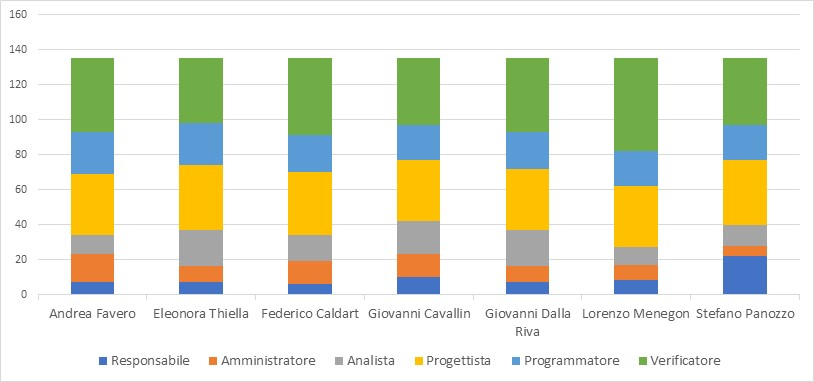
\includegraphics[scale=0.85]{img/Preventivo/Istogrammi/Totale.jpg}}
	\caption{Raffigurazione Prospetto Orario: Riepilogo ore totali}
	\clearpage
\end{figure}
\begin{figure}[H]
	\centerline{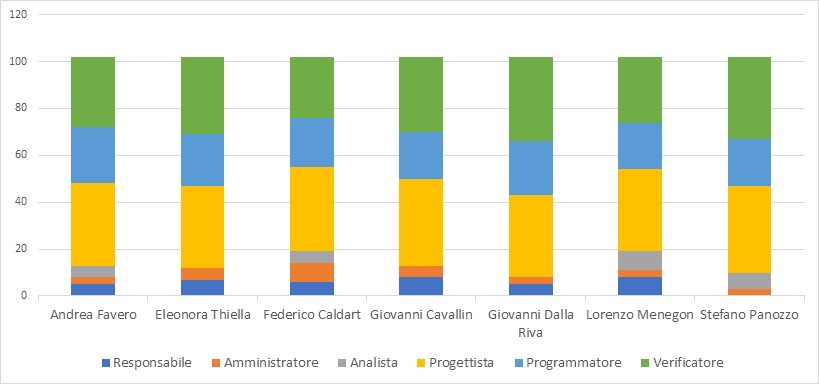
\includegraphics[scale=0.85]{img/Preventivo/Istogrammi/TotaleRendicontato.jpg}}
	\caption{Raffigurazione Prospetto Orario: Riepilogo ore totali rendicontate}
	\clearpage
\end{figure}
\paragraph{Prospetto economico}
Il prospetto economico per l'intera durata del progetto è illustrato in tabella. 
\begin{table}[H]
	\centerline{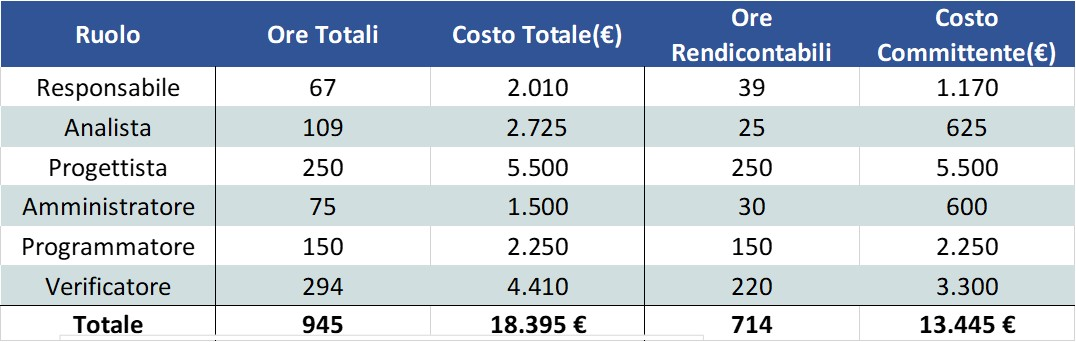
\includegraphics[scale=0.6]{img/Preventivo/TotaleEconomico.jpg}}\label{Totale}
	\caption{Prospetto Economico: Riepilogo}
	\clearpage
\end{table}
\newpage
La raffigurazione grafica del peso di ogni ruolo sul costo totale e rendicontato è così rappresentata: 
\begin{figure}[H]
	\centerline{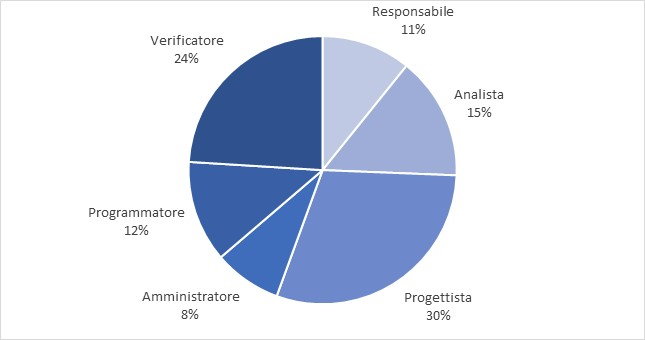
\includegraphics[scale=0.9]{img/Preventivo/Torte/Totale.jpg}}
	\caption{Raffigurazione Prospetto Economico: Riepilogo ore totali}
	\clearpage
\end{figure}
\begin{figure}[H]
	\centerline{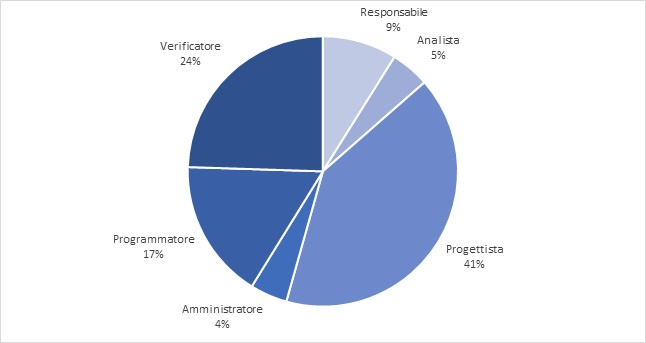
\includegraphics[scale=0.9]{img/Preventivo/Torte/TotaleRendicontato.jpg}}
	\caption{Raffigurazione Prospetto Economico: Riepilogo ore rendicontate}
	\clearpage
\end{figure}

\subsection{Conclusione}
Come si può notare nella \hyperref[Totale]{Tabella 16}, il preventivo finale a carico del committente per il progetto è pari a \EUR{13.445}.
%\newpage
\section{Consuntivo e Preventivo a finire}

In questo capitolo viene effettuato un confronto fra le ore ed il costo preventivati con quelli riscontrati effettivamente durante i periodi del ciclo di sviluppo.
Viene poi analizzato e riportato il bilancio che potrà essere:
\begin{itemize}
	\item \textbf{positivo}: se il consuntivo risulta inferiore o equivalente al preventivo;
	\item \textbf{negativo}: se il consuntivo risulta superiore al preventivo.
\end{itemize}

\subsection{Analisi dei requisiti}
\subsubsection{Consuntivo}
Di seguito è riportata la tabella riassuntiva per il consuntivo del primo periodo
\begin{figure}[h!]
	\centerline{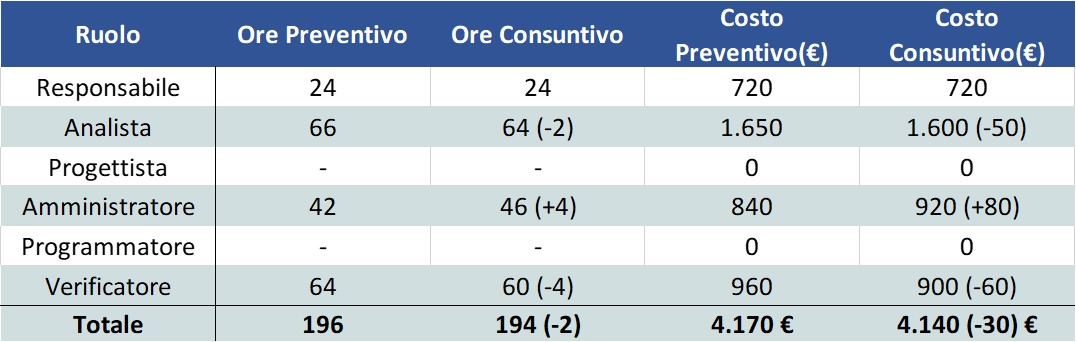
\includegraphics[scale=0.55]{img/Preventivo/AnalisiRequisitiConsuntivo.jpg}}
	\caption{Consuntivo: Analisi dei requisiti}
\end{figure}

\subsubsection{Conclusioni}
In conclusione, durante questo primo periodo non ci sono state grandi discordanze rispetto a quanto pianificato. È possibile visionare i problemi riscontrati nell'\hyperref[RiscontroRischi]{Appendice A} e notare come essi abbiano influito sullo scostamento delle ore totali preventivate e di conseguenza sul costo. Si è inoltre rivelato necessario un impegno minore da parte dei \vers{} rispetto a quanto preventivato.\\
Questi fattori hanno favorito un risparmio rispetto al costo inizialmente preventivato pari a \EUR{30} e quindi il bilancio di questo primo periodo risulta positivo.

\newpage

\section{Attualizzazione dei rischi} \label{RiscontroRischi}

Vengono di seguito analizzati i problemi riscontrati durante lo svolgimento del progetto, suddivisi per ogni periodo; ad ogni occorrenza rilevata corrisponderà una breve descrizione del problema e le contromisure adottate per la sua mitigazione. È inoltre possibile prendere visione di come i problemi qui analizzati abbiano influito sul consuntivo di periodo sul preventivo finale nell'\hyperref[ConsuntivoPeriodo]{Appendice B}.\\

\subsection{Analisi dei requisiti}
\begin{table}[h!]
	\centerline{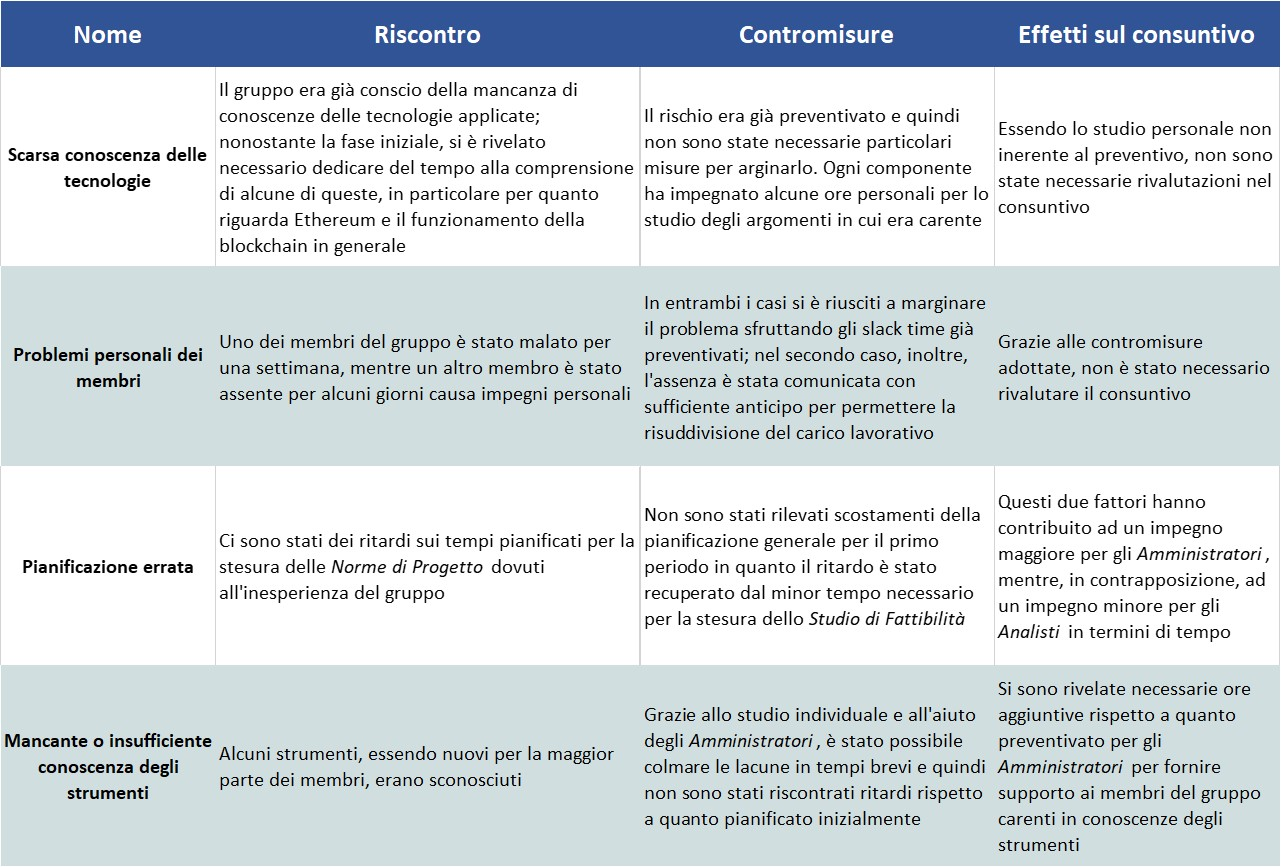
\includegraphics[scale=0.55]{img/Rischi/RiscontroProblemi-AnalisiRequisiti.jpg}}
	\caption{Riscontro problemi: Analisi dei Requisiti}
\end{table}
\clearpage

\subsection{Analisi dei requisiti in Dettaglio} \label{RiscontroAnalisiDettaglio}
\begin{table}[h!]
	\centerline{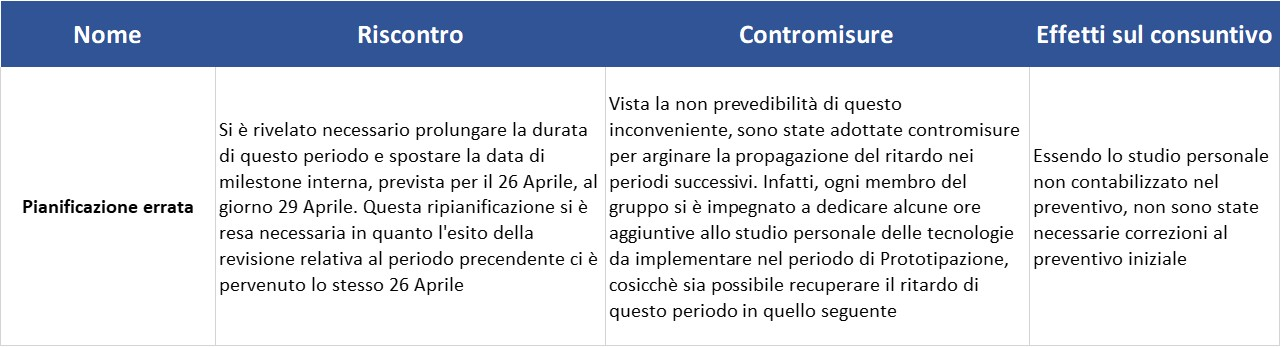
\includegraphics[scale=0.55]{img/Rischi/RiscontroProblemi-AnalisiRequisitiDettaglio.jpg}}
	\caption{Riscontro problemi: Analisi dei Requisiti in Dettaglio}
\end{table}

\subsection{Prototipazione}
\begin{table}[h!]
	\centerline{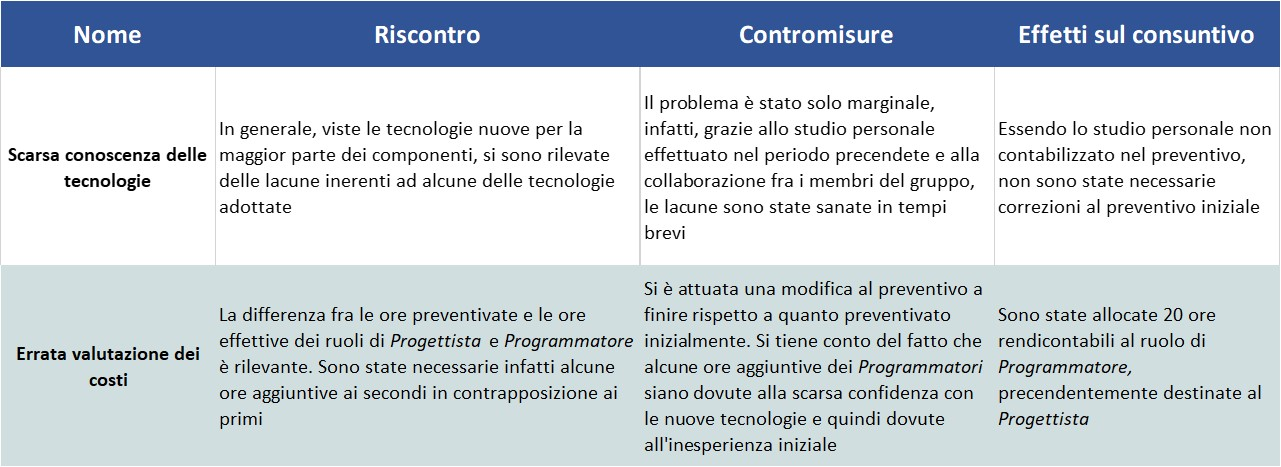
\includegraphics[scale=0.55]{img/Rischi/RiscontroProblemi-Prototipazione.jpg}}
	\caption{Riscontro problemi: Prototipazione}
\end{table}
\clearpage

\subsection{Prototipazione in Dettaglio} \label{RiscontroPrototipazioneDettaglio}
\begin{table}[h!]
	\centerline{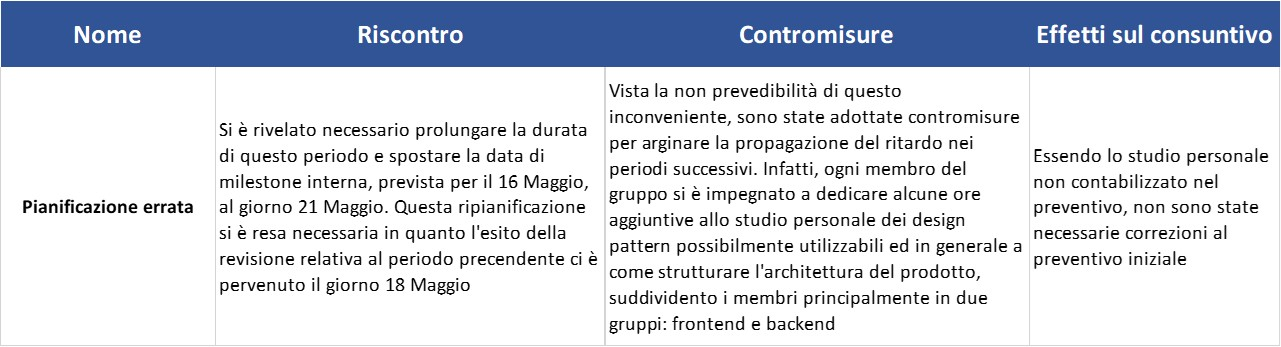
\includegraphics[scale=0.55]{img/Rischi/RiscontroProblemi-PrototipazioneDettaglio.jpg}}
	\caption{Riscontro problemi: Prototipazione in Dettaglio}
\end{table}

\subsection{Progettazione finale e Codifica}
Durante questo periodo non si sono verificati problemi che abbiano influito particolarmente sul perseguimento delle attività pianificate.

%\newpage
\renewcommand{\arraystretch}{1}

\section{Organigramma}

\subsection{Redazione}
\begin{longtable}{ c  c  c }
	\rowcolor{bluSOS}
	\textcolor{white}{\textbf{Nominativo}} & \textcolor{white}{\textbf{Data di redazione}} & \textcolor{white}{\textbf{Firma}}\\
	
	Federico Caldart & 2018-05-06 & 
\includegraphics[height=0.5cm]{img/Firme/FedericoCaldart.png}\\
	\caption{Componente per la redazione}  \\
\end{longtable}

\subsection{Approvazione}
\rowcolors{2}{greySOS}{white}
\begin{longtable}{ c  c  c }
	\rowcolor{bluSOS}
	\textcolor{white}{\textbf{Nominativo}} & \textcolor{white}{\textbf{Data di approvazione}} & \textcolor{white}{\textbf{Firma}}\\
	
	Federico Caldart & 2018-05-06 & 
\includegraphics[height=0.5cm]{img/Firme/FedericoCaldart.png}  \\
	Tullio Vardanega & & \\
	\rowcolor{white}\caption{Componenti per l'approvazione}\\
\end{longtable}

\subsection{Accettazione dei componenti}
\rowcolors{2}{greySOS}{white}
%\cmidrule(r){1-1}\cmidrule(lr){2-2}\cmidrule(l){3-3}
% \raisebox{-\totalheight}{\includegraphics[width=0.3\textwidth, height=60mm]{images/myLboro.png}}

\begin{longtable}{ c  c  c }
	\rowcolor{bluSOS}
	\textcolor{white}{\textbf{Nominativo}} & \textcolor{white}{\textbf{Data di accettazione}} & \textcolor{white}{\textbf{Firma}}\\
	%\includegraphics[height=2.5cm]{immagine} aggiustare l'altezza
	Andrea Favero & 2018-05-06 & 
\includegraphics[height=0.5cm]{img/Firme/AndreaFavero.png} \\
	
	Eleonora Thiella & 2018-05-06 & 
\includegraphics[height=0.5cm]{img/Firme/EleonoraThiella.png} \\
	
	Federico Caldart & 2018-05-06 & 
\includegraphics[height=0.5cm]{img/Firme/FedericoCaldart.png} \\
	
	Giovanni Cavallin & 2018-05-06 & 
\includegraphics[height=0.5cm]{img/Firme/GiovanniCavallin.png} \\
	
	Giovanni Dalla Riva & 2018-05-06 & \includegraphics[height=0.5cm]{img/Firme/GiovanniDallaRiva.png} \\
	
	Lorenzo Menegon & 2018-05-06 & \includegraphics[height=0.5cm]{img/Firme/LorenzoMenegon.png} \\
	
	Stefano Panozzo & 2018-05-06 & \includegraphics[height=0.5cm]{img/Firme/StefanoPanozzo.png} \\
	\rowcolor{white}\caption{Accettazione dei componenti}\\
\end{longtable}


\subsection{Componenti}
\rowcolors{2}{greySOS}{white}
\begin{longtable}{ c  c  c  C{4cm} }
	\rowcolor{bluSOS}
	\textcolor{white}{\textbf{Nominativo}} & \textcolor{white}{\textbf{Matricola}} & \textcolor{white}{\textbf{Indirizzo di posta elettronica}} & \textcolor{white}{\textbf{Ruoli previsti}}\\
	
	Andrea Favero & 1125545 & andrea.favero.8@studenti.unipd.it & \adm, \ana, \prog, \progr, \ver \\
	
	Eleonora Thiella & 1099980 & eleonora.thiella@studenti.unipd.it & \RdP, \prog, \progr, \ver \\
	
	Federico Caldart & 1097005 & federico.caldart.1@studenti.unipd.it & \RdP, \ana, \prog, \progr, \ver \\
	
	Giovanni Cavallin & 1148957 & giovanni.cavallin.1@studenti.unipd.it & \prog, \progr, \ver\\
	
	Giovanni Dalla Riva & 1102075 & giovanni.dallariva@studenti.unipd.it & \adm, \prog, \progr, \ver \\
	
	Lorenzo Menegon & 1097596 & lorenzo.menegon@studenti.unipd.it & \adm, \ana, \prog, \progr \\
	
	Stefano Panozzo & 1097068 & stefano.panozzo.1@studenti.unipd.it & \adm, \ana, \prog, \progr, \ver\\
	\rowcolor{white}\caption{Elenco dei componenti}\\
\end{longtable}
%%%%%%%%%%%%%%%%%%%%%%%%%%%%%%%%%%%%%%%%%%%%%%%%%%%%%%%%%%%%%%%%%%%%%%%%%%%%%%%%%%%%%%%%%%%%%%%%%%%%%%%
\appendix
\pagebreak

\end{document}